\documentclass[twoside]{report}

% ------
% Umlaute
\usepackage{ifluatex,ifxetex}
\ifluatex
  \usepackage{fontspec}
\else
  \ifxetex
    \usepackage{fontspec}
  \else
    \usepackage{selinput}
    \SelectInputMappings{
      adieresis={ä},
      germandbls={ß},
    }
    \usepackage[T1]{fontenc}
    %\usepackage{textcomp}% optional
    %\usepackage{lmodern}
  \fi
\fi

% ------
% Paper auf Deutsch
\usepackage[ngerman]{babel}

% Code Beispiel Java
\usepackage{listings}
\lstset{
	language=Java,
	aboveskip=2mm,
	belowskip=2mm,
	showstringspaces=false,
	columns=flexible,
	basicstyle={\small\ttfamily},
	numbers=none,
	breaklines=true,
	breakatwhitespace=true,
	tabsize=3
}

% ------
% Page layout
\usepackage[hmarginratio=1:1,top=32mm,columnsep=20pt]{geometry}
\usepackage[font=it]{caption}
\usepackage{paralist}
%\usepackage{multicol}


% ------
% Abstract
\usepackage{abstract}
	\renewcommand{\abstractnamefont}{\normalfont\bfseries}
	\renewcommand{\abstracttextfont}{\normalfont\small\itshape}


% ------
% Titling (section/subsection)
\usepackage{titlesec}
\renewcommand\thesection{\Roman{section}}
\titleformat{\section}[block]{\Large\scshape\bfseries}{\thesection.}{1em}{}
\setcounter{secnumdepth}{3}

% ------
% Tabellen über Seitenumbrüche hinweg
\usepackage{longtable}

% ------
% Header/footer
\usepackage{fancyhdr}
	\pagestyle{fancy}
	\fancyhead{}
	\fancyfoot{}
	\fancyhead[C]{Projektdokumentation $\bullet$ PUML $\bullet$ WS18/19$+$SS19}
	\fancyfoot[RO,LE]{}


% ------
% Clickable URLs (optional)
% \usepackage{hyperref}

% ------
% Literaturverweise mit Bibtex einbinden
\usepackage[authoryear,sectionbib,round]{natbib}

% ------
% Bilder laden
\usepackage[pdftex]{graphicx}

% ------
% Maketitle metadata
\title{\vspace{-5mm}%
	\fontsize{24pt}{10pt}\selectfont
	\textbf{Projektdokumentation}
	}	
\author{%
        % alle Autoren hier listen
        % 
	\large
	\textsc{Softwarearchitekt: Philipp Rimmele -- philipp.rimmele@stud.htwk-leipzig.de} \\[2mm]
	\textsc{Autor II -- E-Mail} \\[2mm]
	\textsc{Marian Geißler -- marian.geissler@stud.htwk-leipzig.de} \\[2mm]
	\normalsize	HTWK Leipzig 
	}
\date{}



% Geschachtelte Sections
\newcounter{sectionlevel}

\newcommand{\nsecbegin}[1]
{
    \ifnum\value{sectionlevel} = 0
    \PackageError{nsection}{Die minimale verschachtelungstiefe wurde unterschritten}
    %\part{#1}%
    \else
    \ifcase\value{sectionlevel} 
    \chapter{#1}
    \or
    \section{#1}
    \or
    \subsection{#1}
    \or
    \subsubsection{#1}
    \or
    \paragraph{#1}
    \or
    \subparagraph{#1}
    \else
    \PackageError{nsection}{Die maximale verschachtelungstiefe wurde ueberschritten}
    \fi
    \fi
    \addtocounter{sectionlevel}{1}
}

\newcommand{\nsecend}
{
  \addtocounter{sectionlevel}{-1}
}

\setcounter{sectionlevel}{1}




%%%%%%%%%%%%%%%%%%%%%%%%
\begin{document}


% -------
% Titel und Abstract über beide Spalten
%\twocolumn[
%\begin{@twocolumnfalse}

\maketitle
\thispagestyle{fancy}

\tableofcontents

%%%%
%%%% Die Struktur des Dokuments bitte nicht aendern!!!
%%%%

\nsecbegin{Anforderungsspezifikation}

\nsecbegin{Initiale Kundenvorgaben}
Maecenas sed ultricies felis. Sed imperdiet dictum arcu a egestas. 
In sapien ante, ultricies quis pellentesque ut, fringilla id sem. Proin justo libero, dapibus consequat auctor at, euismod et erat. Sed ut ipsum erat, iaculis vehicula lorem. Cras non dolor id libero blandit ornare. Pellentesque luctus fermentum eros ut posuere. Suspendisse rutrum suscipit massa sit amet molestie. Donec suscipit lacinia diam, eu posuere libero rutrum sed. Nam blandit lorem sit amet dolor vestibulum in lacinia purus varius. Ut tortor massa, rhoncus ut auctor eget, vestibulum ut justo.
\nsecend


\nsecbegin{Produktvision}
Quisque vel arcu eget sapien euismod tristique rhoncus eu mauris. Cum sociis natoque penatibus et magnis dis parturient montes, nascetur ridiculus mus. Cras ligula lacus, dictum id scelerisque nec, venenatis vitae magna. Cras tristique porta elit, non tincidunt ligula placerat lobortis. Pellentesque quam enim, mattis in cursus eu, blandit et massa. Mauris aliquet turpis blandit elit vehicula sed posuere lectus facilisis. Donec blandit adipiscing tortor, quis lobortis purus eleifend vel. Nam a tellus at magna scelerisque blandit vel nec erat.
\nsecend

% Das hier ist ein Absatz, der die Grafik in Abbildung~\ref{fig:bild1} detailliert erläutert, erklärt und interpretiert.

% \begin{figure}[b]
%   \centering
%   \includegraphics[width=4.5cm]{bspbild1.png}
%   \caption{Beispiel für ein einspaltiges Bild}
%   \label{fig:bild1}
% \end{figure}


\nsecbegin{Liste der funktionalen Anforderungen}
XXX
\nsecend

%
% soll der Inhalt dieser Subsection in einer separaten Datei
% (z.B. listefunktional.tex) liegen, dann kann dies mit dem
% folgenden Kommando geschehen.
%
% \input{listefunktional}

\nsecbegin{Liste der nicht-funktionalen Anforderungen}
XXX
\nsecend

\nsecbegin{Weitere Zuarbeiten zum Produktvisions-Workshop}
XXX
\nsecend

\nsecbegin{Zuarbeit von Autor X}
XXX
\nsecend

\nsecbegin{Zuarbeit von Autor Y}
XXX
\nsecend

\nsecbegin{Liste der Kundengespräche mit Ergebnissen}
XXX
\nsecend

\nsecend %Anforderungsspezifikation

\nsecbegin{Architektur und Entwurf}

\nsecbegin{Zuarbeiten der Teammitglieder}
XXX
\nsecend

%Recherche Teil - Marian
\nsecbegin{Commandline Funktionalität}
Eine der Anforderungen an die Software ist die Bedienung des Programms mittels Kommandozeile. Folgende zwei Möglichkeiten scheinen für die Verwendung im Projekt PUML als sinnvoll. Zum einen ist die Parameterabfrage über eine eigene Implementation auf Basis der Hauptklasse möglich mittels \texttt{public static void main(String [] args)}, zum Anderen ist die Nutzung der \glqq Commons CLI\grqq-Bibliothek von Apache eine Option. \\
Während der Recherche zeigte sich, dass die Nutzung der Commons CLI - Bibliothek sehr gut dokumentiert ist und in der Praxis oft Anwendung findet, auch das Umsetzen eines Tests schien weniger problematisch zu gelingen, als ein Abfragen der Parameter über \texttt{String [] args} im Hauptprogramm. Aus diesem Grund wird an dieser Stelle die Apache Bibliothek kurz vorgestellt. \\
Ein Download der Bibliothek erfolgt über die Seite des Enticklers Apache\footnote[1]{http://commons.apache.org/proper/commons-cli/} und muss anschließend in die Entwicklungsumgebung eingebunden, sowie in das Programm importiert werden. \\
Die Arbeit mit Commons CLI lässt sich grundsätzlich in drei Schritte unterteilen, Parameterdefinition, das Einrichten des Parsers und die Verkettung mit der jeweiligen Funktion. \\
Zuerst wird festgelegt, welche Parameter der Anwendung übergeben werden, hierzu wird ein neues Container Objekt vom Typ \texttt{Options} angelegt. Anschließend werden die gewünschten Befehle mit den entsprechenden Parametern dem Container hinzugefügt, so dass später ein Aufruf im Terminal möglich ist, wie bespielsweise \texttt{ls -al meinfile.txt} um die Zugriffsrechte einer Datei zu überprüfen.
\begin{lstlisting}
//Erzeugt neuen Container fuer Programmparameter
Options options = new Options();
//Hinzufuegen einer neuen Option 
options.addOption("l",false, "Alle Leerzeichen entfernen.");
\end{lstlisting}
Zunächst wird ein Parser intitialisert, während anschließend über eine logische Verknüpfung der Flags die entsprechende Funktion aufgerufen wird. Wichtig ist in diesem Zusammenhang noch die Verwendung von Exceptions zu erwähnen, die entweder durch den Ausdruck \texttt{ParseException} aus der Bibliothek oder \texttt{try / catch} Schlüsselwörter abgefangen werden müssen.
\begin{lstlisting}
CommandLineParser parser = new DefaultParser();	
CommandLine commandLine = parser.parse(options,args);

 if(commandLine.hasOption("b"))
{
	System.out.println("String eingebe: ");
	String myString = keyboard.nextLine();	//String einlesen
	getWordBefore('.',myString); // liefere alle Woerter vor Punkt
}
if (commandLine.hasOption("l"))
{
	String myString = "g e s p e r r t g e s c h r i e b e n";
	System.out.println(noSpace(myString));	//entfernt alle Leerzeichen
}
\end{lstlisting}
Am Ende muss das Programm übersetzt werden und steht anschließend zur Nutzung mit den gesetzten Parametern zur Verfügung. So liefert in diesem Fall die Eingabe im Terminal: \texttt{java MeinProgrammName -l } die Ausgabe \glqq gesperrtgeschrieben\grqq zurück.
\nsecend

\nsecbegin{Entscheidungen des Technologieworkshops}
XXX
\nsecend

\nsecbegin{Überblick über Architektur}
XXX
\nsecend

\nsecbegin{Definierte Schnittstellen}
XXX
\nsecend

\nsecbegin{Liste der Architekturentscheidungen}
XXX (bewusste und unbewusste Entscheidungen mit zeitlicher Einordnung)
\nsecend


\nsecend %Architektur und Entwurf

\nsecbegin{Prozess- und Implementationsvorgaben}

\nsecbegin{Definition of Done}
XXX
\nsecend

\nsecbegin{Coding Style}
Bitte die Datei javaCodeStyle.xml im specification-Verzeichniss in Eclipse importieren und verwenden.
Hierfür in Eclipse unter "`Window->Preferences->Java->Code Style->Formatter"' auf Import klicken und die XML-Datei auswählen.\\
Ist der passende Coding Style eingestellt kann der Quellcode mit "`STRG+SHIFT+F"' automatisch formatiert werden.
Wird dies vor jedem Commit gemacht, ensteht ein einheitlicher Code-Style und die Änderungen können gut mit GIT überprüft werden.\\
\begin{figure}[hbtp]
\centering
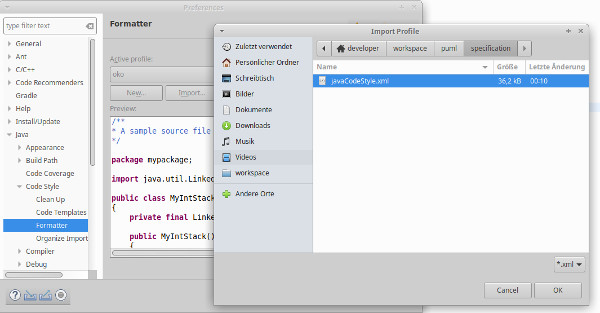
\includegraphics[scale=0.5]{Bilder/importCodeStyle}
\caption{Code-Style in Eclipse importieren}
\end{figure}
Des weiteren empfielt es sich bei größeren oder stark geschachtelten Code-Abschnitten die Zugehörigkeit der Schließenden Klammer mit einem Kommentar zu Kennzeichnen.\\
Sonstige Konventionen:
\begin{itemize}
\item{Variablen und Instanzen beginnen kleingeschrieben}
\item{Klassen und Interfaces beginnen mit Großbuchstaben}
\item{Besteht ein Namen aus mehreren zusammengesetzten Wörtern, beginnen alle weiteren Wörter mit Großbuchstaben (keine Unterstriche in Namen verwenden)}
\item{Aussagekräftige Namen verwenden}
\item{Alle Namen auf Englisch}
\item{Die Kommentare auf Deutsch}
\end{itemize}

\nsecend

\nsecbegin{Zu nutzende Werkzeuge}
\begin{itemize}
\item{Eclipse - Entwicklungsumgebung}
\item{GIT - Dateiversionierung}
\item{Meld - Unterschiede zwischen Dateien anzeigen}
\item{Texmaker - Latex-Editor}
\item{GIMP - Bildbearbeitung für das Editieren von Screenshots}
\end{itemize}
\nsecend



\nsecend %Prozess- und Implementationsvorgaben

%%%%%%%%%%%%
%% Abschnitt mit den Sprints beginnt hier
%%%%%%%%%%%%

\nsecbegin{Sprint 1}

\nsecbegin{Ziel des Sprints}
Es soll eine funktionsfähige Basisversion, welche für das einfache erstellen von Klassendiagrammen aus Java-Code verwendet werden soll entstehen. Das Programm soll sowohl über die Kommandozeile, als auch über eine grafische Oberfläche bedient werden können. Die erzeugten Klassendiagramme sollen in der grafischen Oberfläche angezeigt werden können.

\begin{figure}[hbtp]
\centering
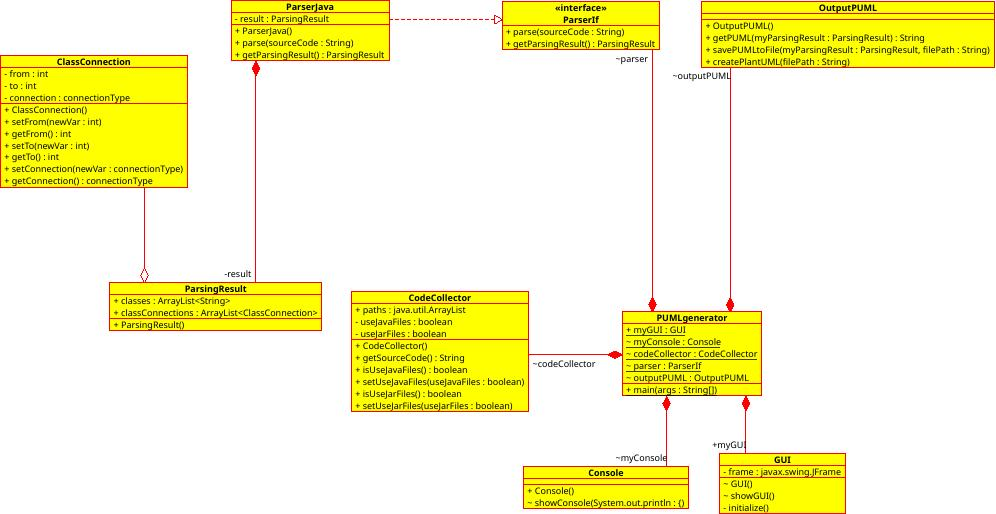
\includegraphics[scale=0.5]{Bilder/classDiagrammSprint1}
\caption{Klassendiagramm des Sprints}
\end{figure}
\nsecend

\nsecbegin{User-Stories des Sprint-Backlogs}
\nsecbegin{Dateien einlesen}
\nsecbegin{Art der eingelesenen Datei}
Als Benutzer wünsche ich mir, dass eine Auswahl zwischen Jar- und Java-Dateien möglich ist, damit Quellcode nicht doppelt eingelesen wird.
\nsecend

\nsecbegin{Java-Dateien}
Als Benutzer wünsche ich mir, dass Java-Dateien einlesbar sind, um den Quellcode von einer oder mehreren Klassen zu analysieren.
\nsecend

\nsecbegin{Jar-Dateien}
Als Benutzer wünsche ich mir, dass Jar-Dateien einlesbar sind, um den Quellcode zu analysieren.
\nsecend
\nsecend

\nsecbegin{Vorschau}
Als Benutzer wünsche ich mir eine Vorschau der Diagramme, damit ich einschätzen kann ob ich damit zufrieden bin.
\nsecend

\nsecbegin{Kommandozeile}
Als Benutzer wünsche ich mir, dass das Programm von der Kommandozeile aus aufrufbar ist, um es automatisiert starten zu können.
\nsecend

\nsecbegin{Klassendiagramme}
Als Benutzer wünsche ich mir, Klassendiagramme aus meinem bestehenden Quellcode erstellen zu können, damit ich das nicht manuell tun muss.
\nsecend

\nsecbegin{Anzeigen und Speichern von PlantUML}
Als Benutzer wünsche ich mir, Diagramme als PlantUML-Code anzeigen und speichern zu können, um den Aufbau nachvollziehen zu können.
\nsecend

\nsecbegin{Plattformunabhängigkeit}
Als Project Owner wünsche ich mir, dass das Programm plattformunabhängig ist, damit es sich gut verbreiten lässt.
\nsecend

\nsecend

\nsecbegin{Liste der durchgeführten Meetings}
\begin{itemize}
\item Planning-Meeting
\end{itemize}
\nsecend

\nsecbegin{Ergebnisse des Planning-Meetings}
Dem gesammten Team ist die geplante Grundstruktur des Programms bekannt. Jeder weis welchen Teil des Programms er implementieren soll.
\nsecend

\nsecbegin{Aufgewendete Arbeitszeit pro Person$+$Arbeitspaket}
\begin{longtable}{|p{4cm}|l|l|l|l|l|}
        \hline
        Arbeitspaket & Person & Start & Ende & h & Artefakt\\
        \hline
        Dummyklassen & Musterstudi & 3.5.09 & 12.5.09 & 14 & Klasse.java\\ \hline
        AP XYZ &  &  &  & & \\ \hline
\end{longtable}     
\nsecend

\nsecbegin{Konkrete Code-Qualität im Sprint}
XXX
\nsecend

\nsecbegin{Konkrete Test-Überdeckung im Sprint}
XXX
\nsecend

\nsecbegin{Ergebnisse des Reviews}
XXX
\nsecend

\nsecbegin{Ergebnisse der Retrospektive}
XXX
\nsecend

\nsecbegin{Abschließende Einschätzung des Product-Owners}
XXX
\nsecend

\nsecbegin{Abschließende Einschätzung des Software-Architekten}
XXX
\nsecend

\nsecbegin{Abschließende Einschätzung des Team-Managers}
XXX
\nsecend


\nsecend

\nsecbegin{Sprint 2}
%% %Autoren: Julian Uebe, Jan Sollmann
\nsecbegin{Ziel des Sprints}
Dieser Sprint ist ausschließlich dazu gedacht, im Verlauf des ersten Sprints identifizierte und noch nicht behobene Bugs zu entfernen. Es wurden bewusst keine neuen User-Stories (für den Benutzer) im Sprint-Backlog definiert. Der Fokus liegt darauf, die im ersten Sprint geschaffene Basis noch einmal zu stabilisieren.
\nsecend

\nsecbegin{User-Stories des Sprint-Backlogs}
\nsecbegin{Reduzierung von Bugs}
Als Softwarearchitekt und Product Owner wünschen wir uns, dass möglichst wenige Bugs auftreten, um die spätere Weiterentwicklung und damit die uneingeschränkte Funktionalität des Produkts nicht zu gefährden.
\nsecend
\nsecend % {User-Stories des Sprint-Backlogs}

\nsecbegin{Zeitliche Planung}
\begin{figure}[hbtp]
\centering
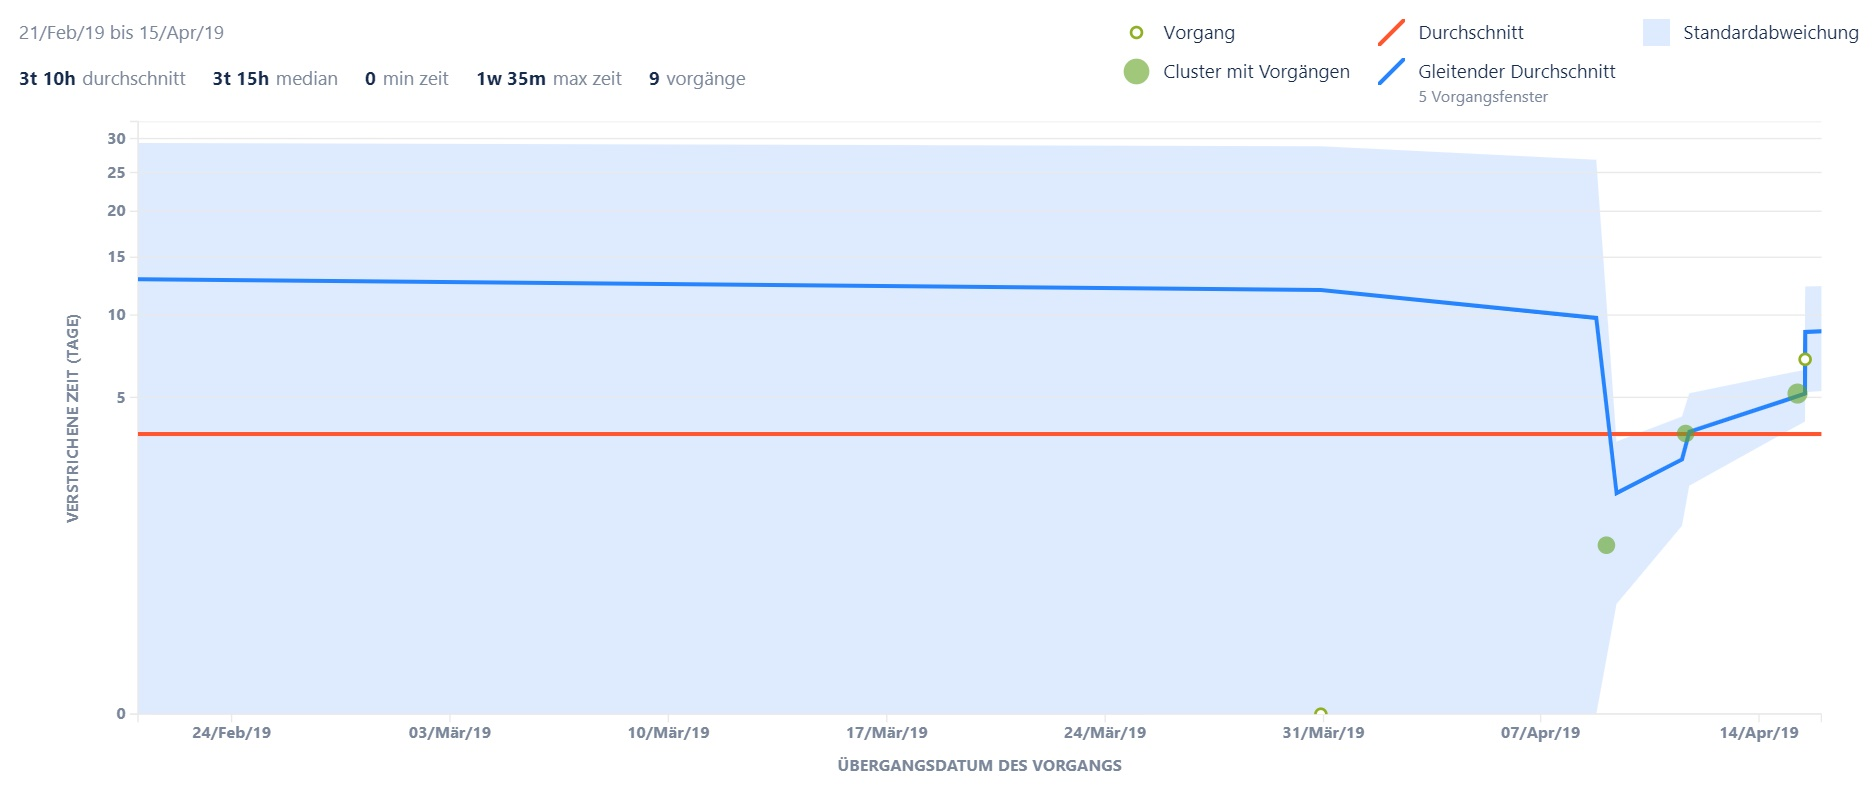
\includegraphics[width=\textwidth]{Bilder/diagram_sprint2}
\caption{Kontroll-Diagramm für Sprint 2}
\end{figure}
\nsecend%Zeitliche Planung

\nsecbegin{Liste der durchgeführten Meetings}
\begin{itemize}
\item Planning-Meeting (21.02.2019)
\item Zwischen-Meeting (08.04.2019)
\item Zwischen-Meeting (11.04.2019)
\item Review-Meeting (15.04.2019)
\end{itemize}
\nsecend%Liste der durchgeführten Meetings

\nsecbegin{Ergebnisse des Planning-Meetings}
Der zweite Sprint wird zeitlich in der letzten Woche der Semesterferien begonnen und bis zum Ende der ersten Woche der Vorlesungszeit gehen. Dies wurde mit den Teammitgliedern besprochen. Hauptziel des Sprints ist ein sauberer Stand, mit dem ab dem kommenden Sommersemester weitergearbeitet werden kann.
\nsecend

\nsecbegin{Aufgewendete Arbeitszeit pro Person$+$Arbeitspaket}
\begin{longtable}{|p{4cm}|l|l|l|l|l|}
        \hline
        Arbeitspaket & Person & Start & Ende & h & Artefakt\\
        \hline
        Testdaten & Marian Geissler   & 06.04.2019 & 15.04.2019 & 2 &  \\ \hline
        Logger & Patrick Otte   & 08.02.2019 & 08.04.2019 & 12 & LogMain.java \\ \hline
        Output & Patrick Otte   & 11.04.2019 & 15.04.2019 & 3 & OutputPUML.java \\ \hline
        Konsole & Johann Gerhardt   & 14.04.2019 & 14.04.2019 & 1 & Console.java \\ \hline
        Java-Parser & Michael Lux   & 30.03.2019 & 30.03.2019 & 14 & ParserJava.java\\ \hline
        GUI & Jan Sollmann  & 01.04.2019 & 06.04.2019 & 5 & GUI\_SWT.java \\ \hline
        GUI & Julian Uebe  & 21.02.2019 & 15.04.2019 & 7 & SWT-Tool \\ \hline
        Code-Collector & Elisabeth Schuster  & 07.02.2019 & 14.04.2019 & 5.5  & CodeCollector.java \\ \hline
        Profiler & Elisabeth Schuster  & 10.04.2019 & 26.04.2019 & 7  & Profiler \\ \hline
       Java-Parser & Jona Meyer  & 30.03.2019 & 30.03.2019 & 7 & ParserJave.java \\ \hline
        Code-Collector & Leo Rauschke  & 07.04.2019 & 14.04.2019 & 5.75 & CodeCollector.java \\ \hline
        Profiler & Leo Rauschke  & 09.04.2019 & 29.04.2019 & 3 & Profiler\\ \hline
        Output & Tore Arndt  & 11.04.2019 & 15.04.2019 & 5 & OutputPUML.java\\ \hline
        
        
\end{longtable}     
\nsecend

\nsecbegin{Konkrete Code-Qualität im Sprint}
Die Codequalität ist etwas besser geworden. Wobei hin und wieder durchaus noch massive Unschönheiten bemängelt werde müssen.
\nsecend

\nsecbegin{Konkrete Test-Überdeckung im Sprint}
Die Testüberdeckung ist auf 40,6\% gesunken.
\nsecend

\nsecbegin{Ergebnisse des Reviews}
\begin{table}[H]

\begin{tabularx}{\textwidth}{ |l|l|X| }
\hline
\textbf{Klasse} & \textbf{Methode} & \textbf{Anmerkungen}\\
 \hline
 
 Testdatensatz & komplett & zukünftig als automatischer Ausgabe-Test\\ \hline
 GUI\_SWT.java & komplett & wird durch Swing-GUI ersetzt\\ \hline
 CodeCollector & Pfadbehandlung & Funktioniert nun auch unter Windows\\ \hline
 CodeCollector & einlesen & Funktioniert\\ \hline
 ParserJava.java & buildTree & Es bestehen weitherhin Bugs\\ \hline
 Alle & komplett & Unit-Tests für das ganze Programm folgen\\ \hline
 ParserJava.java & buildTree & Erweiterung für das Erstellen von Sequenzdiagrammen\\ \hline
 GUI\_SWT.java & createContents, runPUML & Ausgabe für Sequenzdiagramme muss implementiert werden\\ \hline
 
%Console & showConsole & Pfad anpassen \\
\hline
\end{tabularx}
\end{table}

\nsecend%Ergebnisse des Reviews

\nsecbegin{Ergebnisse der Retrospektive}
Die Retrospektive schloss mit einer positiven Bilanz. (...)
\nsecend%Ergebnisse der Retrospektive

\nsecbegin{Abschließende Einschätzung des Product-Owners}
In diesem Sprint wurden einige kritische Bugs behoben und somit User Stories des letzten Sprint-Backlogs noch vervollständigt. Zu hoffen bleibt trotzdem, dass in allen folgenden Sprints auch neue Funktionalität hinzugefügt wird.
\nsecend%Abschließende Einschätzung des Product-Owners

\nsecbegin{Abschließende Einschätzung des Software-Architekten}
Der erste Meilenstein wird als erreicht angesehen, auch wenn der Parser durchaus noch Mängel enthält. Der Grundentwurf der Architektur ist vollständig umgesetzt. Da im nächsten Sprint die Sequenz-Diagramme hinzugenommen sollen, wird hier ein kleiner Umbau der Architektur notwendig sein. Die Klassen ParsingResult, welche nur Daten (unter anderem vom Typ ClassConnection) enthält wird durch XML ersetzt. Dies war von Anfang an vorgesehen, wurde aber aufgrund der höheren Komplexität bisher vermieden. Des weiteren haben wir beschlossen die Sprintdauer auf 2 Wochen zu verkürzen, um die Entwicklung zu beschleunigen.
\nsecend%Abschließende Einschätzung des Software-Architekten

\nsecbegin{Abschließende Einschätzung des Team-Managers}
Insgesamt kann positiv herausgehoben werden, dass sich die Teammitglieder geschlossen dazu bereit erklärten, Teil ihrer Semesterferien für den zweiten Sprint zu opfern. Die Motivation, das Produkt weiter voranzubringen, scheint derzeit ungebrochen.
\nsecend%Abschließende Einschätzung des Team-Managers
\nsecend

%%%%%% weitere Sprints analog


\nsecbegin{Dokumentation}

\nsecbegin{Handbuch}
XXX
\nsecend

\nsecbegin{Installationsanleitung}
XXX
\nsecend

\nsecbegin{Software-Lizenz}
XXX
\nsecend

\nsecend %Dokumentation


\nsecbegin{Projektabschluss}

\nsecbegin{Protokoll der Abnahme und Inbetriebnahme beim Kunden}
XXX
\nsecend

\nsecbegin{Präsentation auf der Messe}
Poster, Bericht
\nsecend

\nsecbegin{Abschließende Einschätzung durch Product-Owner}
XXX
\nsecend

\nsecbegin{Abschließende Einschätzung durch Software-Architekt}
XXX
\nsecend

\nsecbegin{Abschließende Einschätzung durch Team-Manager}
XXX
\nsecend


\nsecend %Projektabschluss

\end{document}
